In addition to the regular spin-down of radio pulsars due to magnetic braking, some
pulsars undergo anomalies in their timing solutions known as \emph{glitches}.
\citet{Edwards2006} describes how these can be modelled by a permanent increase
in the phase, frequency, and first frequency derivative in addition to a
frequency increment that subsequently decays exponentially to zero. That is,
Eqn.~\eqref{eqn: Taylor compact} picks up an additional term
\begin{align}
\phi_{\textrm{g}} = \left\{
\begin{array}{ll}
\Delta\phi + \Delta\nu(\tTOA - \tg) + \frac{1}{2}\Delta\dot{\nu}(\tTOA - \tg)^{2}
+ \left[1-\textrm{e}^{-(\tTOA - \tg)/\tau}\right]\Delta\nu_{\textrm{t}}(\tTOA - \tg)
& \tTOA \ge \tg \\
0 & \tTOA < \tg
\end{array}
\right.
\label{eqn: glitch timing model}
\end{align}
for each modelled glitch. The first three terms are the permanent increase
in phase, frequency, and spin-down, while the last term gives the transient
increase in the frequency $\Delta\nu_{\textrm{t}}$ which decays exponentially
with a timescale $\tau$. In effect this means that pulsar astronomers fit
separate a Taylor expansions either side of the glitch. Due to the fact that
the rise time over which glitch occurs is short compared to the frequency
with which observers take measurements, timing solutions can not resolve the
detailed variation which occur during the glitch: they are limited to describing
the global behaviour before and after.

Fitting this model, pulsar astronomers find that glitches are sudden positive
jumps in the frequency $\Delta\nu > 0$, with typical values of $10^{-9}$~Hz to
$10^{-4}$~Hz; for some pulsars this is accompanied by a change, with either
sign, in the spin-down which has absolute magnitudes between $10^{-19}$~Hz/s to
$10^{-12}$~Hz/s. A comprehensive review of glitches was carried out by
\citet{Espinoza2011} and to illustrate a typical glitch we present a figure
from this work in Fig.~\ref{fig: glitch}.
\begin{figure}[htb]
    \centering
    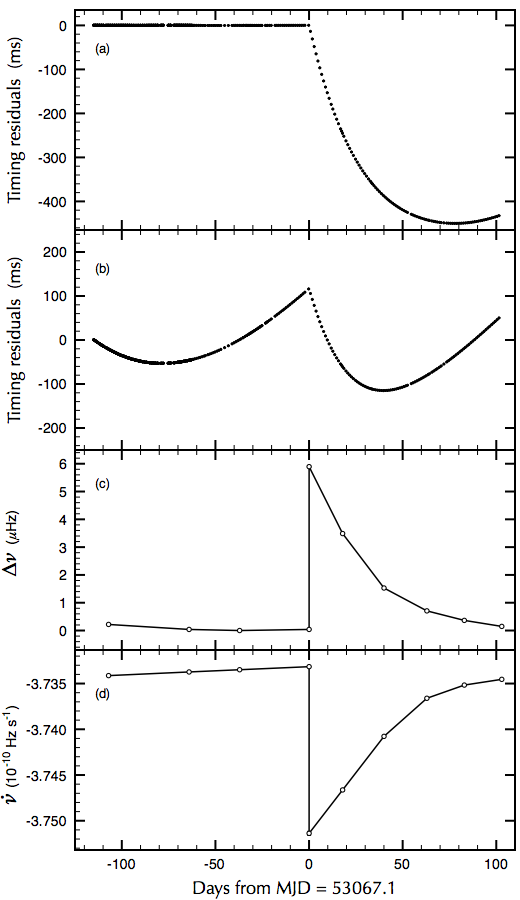
\includegraphics[width=0.5\textwidth]{GlitchExample_jbman}
    \caption{
A glitch in the data of PSR B0531+21, the Crab pulsar. It occurred around MJD
53067 and had a fractional frequency jump of $\Delta\nu/\nu = 5.33 \pm 0.05
\times 10^{−9}$; a small glitch. (a) The timing residuals relative to a
slowdown model with two frequency derivatives when fitting data only up to the
glitch date. (b) Timing residuals after fitting all data in the plot; note
that the glitch feature is still visible. Both these panels have the same
scale, cov- ering 500 ms. (c) Frequency residuals, obtained by subtracting the
main slope given by an average $\dot\nu$.  (d) The behaviour of $\dot\nu$
through the glitch. This figure and caption are taken from Fig.~1 of
\citet{Espinoza2011}}
    \label{fig: glitch}
\end{figure}

Eqn.~\eqref{eqn: glitch timing model} models the glitch with a so-called recovery
consisting of a fraction $Q$ of the initial frequency jump which decays over
a timescale $\tau$ leaving only the permanent increase in frequency. A review
including measurements of this was conducted by \citet{Lyne2000}; they found
that in glitches from 18 pulsars, $Q$ correlates with $|\dot{\nu}|$ reaching
values as large as $\sim0.9$ for the youngest pulsar with the highest absolute
spin-down rate, PSR~B0531+21 also known as the Crab pulsar.

Many pulsars have been observed to glitch several times, \citet{Melatos2008}
considered the waiting times between glitches and concluded that in most
glitching pulsars the glitches happen randomly with waiting times consistent
with a Poisson process, except in PSR J0537-6910 and PSR J0835-4510 which
displayed quasi-periodicity in the waiting times.

In Chapter~\ref{sec: glitches in cgw} we perform our own investigation into the
population statistics of glitches with an aim to understand their implication
for gravitational wave searches. We find, in agreement with
\citet{Espinoza2011} and references therein, that the distribution of glitch
magnitudes has multiple modes which suggests that glitches may come from more
than one mechanism. We go on to apply a statistical model and determine, in an
empirical fashion, the properties of the underlying source populations.

Glitches provide a unique opportunity to investigate the physics of neutron
stars and many of the leading insights have been gained by their study. Two
leading models exist known as the \emph{superfluid unpinning} model and the
\emph{starquake} model.

In the superfluid unpinning model proposed by \citet{Anderson1975}, the star
contains a superfluid component in which the angular momentum is stored in an
array of vortices which are `pinned' to the crust. The magnetic dipole is
frozen into the crust and exerts a torque on the crust, gradually spinning it
down. The superfluid component cannot decrease its angular momentum without
destroying its vortices and so does not spin-down at the same rate.  A lag in
frequency between the superfluid component and rest of the crust develops until
the forces are sufficiently large to cause an avalanche of unpinning events
rapidly transferring the stored angular momentum in the superfluid component to
the crust. The observed pulsations measure the rotation rate of the crust into
which the dipole is frozen, so when this unpinning occurs, we see a rapid
increase in the frequency.

The second model, starquakes, follows from the observation that a rapidly
spinning fluid body has an oblate `rest shape' with a bulge about its equator
due to the centrifugal force. The crust of a star spinning at a frequency $\nu_0$
will solidify with a corresponding oblateness. Subsequently, as the star spins down,
it will have a different rest shape due to its decreased frequency, but the crust
will retain a memory of the earlier shape at which it solidified. This will cause
strains in the crust which eventually cause a starquake relieving the strain,
resetting the reference rest shape, and producing glitch like features.

Both of these models have support in the literature and have been developed
significantly to explain the variety of observed glitches. However, there are
observations which cause difficulties for both models: glitches seen in the
Vela pulsar are too large and too often to be consistent with a starquakes
model, while the unpinning model requires a superfluid component which is at
odds with observation of precession (we discuss this further in
Chapter~\ref{sec: testing models}).


